% Define the page style
\fancypagestyle{chapterstyle}{
   \fancyhead[L]{\nouppercase{\rightmark}}
   \fancyhead[R]{Projet de fin d'etudes 2023-2024}
   \fancyfoot[C]{\vspace{20pt}\thepage} % Adjust the vertical space here
   \setlength{\headheight}{20pt}
   \setlength{\footskip}{30pt} % Adjust the value as needed
}


\chapter{Analyse et Spécifications des besoins}
\pagestyle{chapterstyle}
Dans ce chapitre, nous menons une étude approfondie du processus existant en mettant
en évidence les solutions de gestion de recrutement actuellement adoptées par 4D, ainsi
que les plateformes et les outils qui existent déjà sur le marché. Cela est dans l’objectif
de cerner les besoins fonctionnels et non fonctionnels auxquels doit répondre le projet.

\newpage
\vspace{1cm}

%-------------Spécifications des exigences-----------

\section{Analyse de l'existant}
Actuellement, chez 4D, il n’existe pas de plateforme centralisée pour gérer le processus
de recrutement. Les recruteurs utilisent plusieurs outils qui varient selon les différentes
étapes du processus, incluant LinkedIn, Gmail entre autres. Cette diversification des outils
entraîne plusieurs problèmes tels que le risque de perte d’informations, des difficultés de
coordination, ainsi qu’un temps de traitement des candidatures plus élevé. Ce processus
passe en fait par plusieurs étapes, notamment :

\begin{enumerate}
   \item \textbf{Publication des annonces :} le processus de recrutement débute par la publication des offres d’emploi sur LinkedIn. Les recruteurs de 4D rédigent des annonces
   détaillées incluant les qualifications requises, les responsabilités du poste, ainsi que
   les informations sur l’entreprise. Ces annonces contiennent une adresse e-mail dédiée
   où les candidats peuvent envoyer leurs candidatures..
   \item \textbf{Réception des candidatures :} Les candidats intéressés par les postes publiés
   envoient leur dossier de candidature par e-mail à l’adresse fournie dans l’annonce. Ce
   dossier comprend généralement un CV et une lettre de motivation. Les candidatures
   sont ensuite centralisées dans une boîte de réception gérée par les recruteurs.
   
   \item \textbf{Traitement manuel des candidatures :} Les recruteurs examinent manuellement
   chaque candidature reçue. Ils évaluent les CVs et les lettres de motivation pour
   déterminer si les candidats répondent aux critères du poste. Cette phase implique
   une analyse approfondie des compétences et de l’expérience des candidats et peut
   être sujette à des risques d’erreurs humaines, d’oublis ou de retards.
   
   \item \textbf{Planification des entretiens :} Une fois les candidatures présélectionnées, les recruteurs contactent les candidats par e-mail pour organiser des entretiens oraux
   sans qu’il y ait des tests techniques écrits pour mieux évaluer les compétences des
   candidats. À ce stade, ils utilisent l’application Calendly. Il s’agit d’un outil de planification en ligne qui permet de synchroniser les agendas des recruteurs avec les
   disponibilités des candidats. Les recruteurs envoient un lien Calendly aux candidats,
   leur permettant de choisir un créneau horaire parmi ceux disponibles.
   \item \textbf{Programmation des réunions :} Après que les candidats ont sélectionné leur
   horaire de disponibilité via Calendly, les recruteurs programment les entretiens de
   façon manuelle sur Zoom. Ils créent une réunion pour chaque entretien prévu et
   envoient le lien de la réunion aux candidats.
   \item \textbf{Réalisation des entretiens :}  Les entretiens se déroulent à la date et à l’heure
   convenues, via Zoom. Les candidats, qui sont sélectionnés, sont informés par e-mail
   afin qu’ils entament le processus d’intégration.
   
\end{enumerate}

En bref, le processus de recrutement actuel chez 4D repose sur une série d’étapes qui
nécessitent beaucoup d’interventions humaines. De ce fait, il pourrait avoir des améliorations et bénéficier d’une digitalisation plus automatisée et intégrée. Le diagramme BPMN
suivant résume l’ensemble des étapes du processus :

\begin{figure}[h]
   \centering
   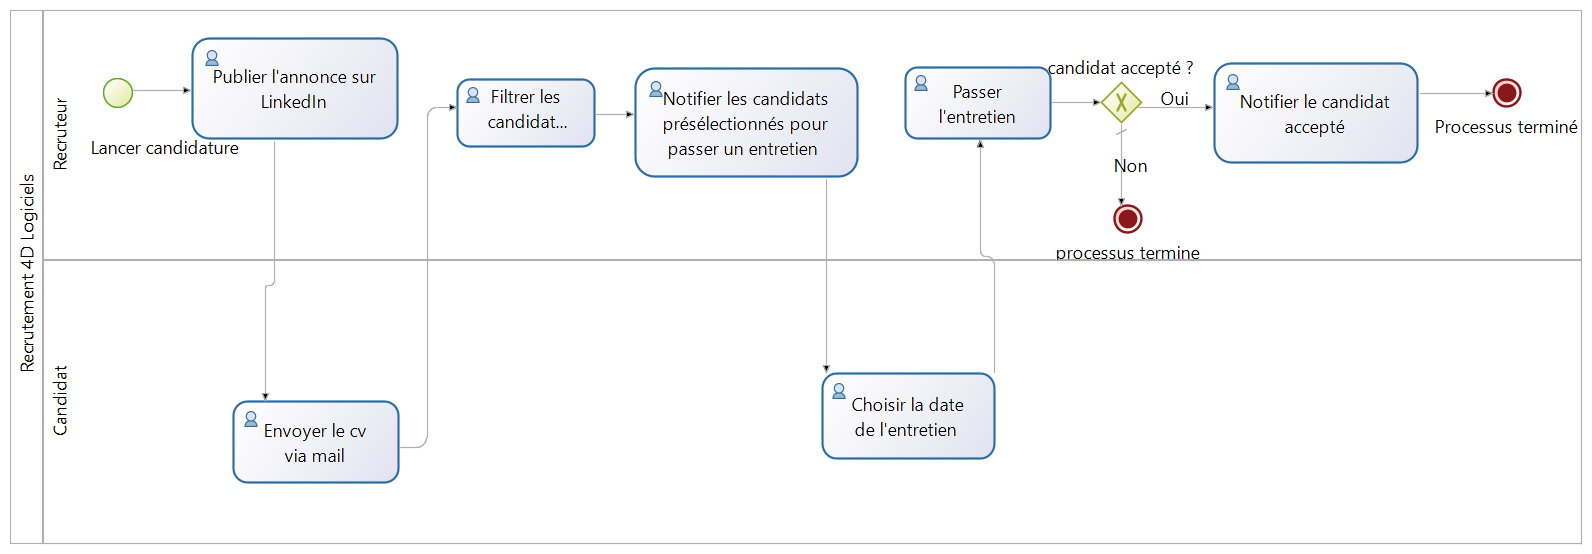
\includegraphics[scale=0.3]{Images/BPMN1.png} 
   \caption{Diagramme BPMN du processus actuel de recrutement chez 4D}
   \label{fig:BPMN1}
\end{figure}




%--------- Benchmarking ----------

\section{Benchmarking des principales solutions de recrutement}
\subsection{Solutions existantes sur le marché}

Il existe une multitude de plateformes qui sont destinées à la gestion de recrutement
et qui proposent une variété de fonctionnalités qui facilitent ce processus. Parmi ces plateformes, nous citons :


{\small % Début de la taille de police small
\renewcommand{\arraystretch}{1.5}
\begin{longtable}{|p{2cm}|p{4.5cm}|p{4cm}|p{4.2cm}|}
\caption{Comparaison des solutions de recrutement} \\
\hline
\rowcolor{blue!30}
\textbf{Solution} & \textbf{Fonctionnalités principales} & \textbf{Avantages} & \textbf{Inconvénients} \\
\hline
\textbf{Indeed} & 
\begin{minipage}[t]{5cm}
- Publication d'offres \\ 
d'emploi \\
- Recherche de CV \\
- Campagnes sponsorisées\\
\end{minipage} &
\begin{minipage}[t]{5cm}
- Grande popularité \\
- Facilité d'utilisation
\end{minipage} &
\begin{minipage}[t]{5cm}
- Qualité variable\\
 des candidats \\
- Options limitées sans\\ 
paiement
\end{minipage} \\
\hline
\textbf{LinkedIn Recruiter} & 
\begin{minipage}[t]{5cm}
- Recherche avancée \\ 
de candidats \\
- Gestion des talents \\
- Analyses et rapports\\
\end{minipage} &
\begin{minipage}[t]{5cm}
- Large base de \\
données de candidats \\
- Outils de sourcing \\ 
puissants
\end{minipage} &
\begin{minipage}[t]{5cm}
- Coût élevé \\
- Complexité d'utilisation\\ 
pour les débutants
\end{minipage} \\
\hline
\textbf{Rekrute} & 
\begin{minipage}[t]{5cm}
- Publication d'offres \\ 
d'emploi \\
- Base de données de CV \\
- Solutions RH intégrées
\end{minipage} &
\begin{minipage}[t]{5cm}
- Forte présence en \\
Afrique du Nord \\
- Interface adaptée\\ 
aux marchés locaux
\end{minipage} &
\begin{minipage}[t]{5cm}
- Moins connu en dehors \\ 
des marchés ciblés \\
- Options limitées pour les \\
entreprises internationales\\

\end{minipage} \\
\hline
\textbf{Odoo:  Module de recrutement} & 
\begin{minipage}[t]{5cm}
- Suivi des candidatures \\
- Intégration avec autres \\ 
modules Odoo \\
- Personnalisation des \\
processus de recrutement
\end{minipage} &
\begin{minipage}[t]{5cm}
- Intégration complète\\ 
avec l'écosystème Odoo \\
- Grande flexibilité \\ 
et personnalisation
\end{minipage} &
\begin{minipage}[t]{5cm}
- Complexité de \\ 
configuration initiale \\
- Nécessite des \\ 
compétences techniques \\ 
pour la personnalisation\\
\end{minipage} \\
\hline
\end{longtable}
} % Fin de la taille de police small


\subsection{Synthèse de l’étude benchmarking}
Cette étude comparative nous a conduits à remarquer clairement 
l'insuffisance des différentes solutions de recrutement disponibles 
sur le marché. Certaines répondent aux besoins fonctionnels liés 
seulement aux modules administratifs, et d’autres présentent des 
complexités liées au déploiement et à l’installation. De plus, 
la plupart des solutions sont fermées à l’introduction de nouvelles 
fonctionnalités, révélant une absence totale de l’aspect évolutif des 
systèmes. D'où l’intérêt de penser à une solution moderne avec un aspect 
modulaire, évolutif, et en responsive design.

\subsection{Pourquoi créer une plateforme de recrutement pour 4D}
Apres avoir étudier le marché de recrutement en ligne et en faisant l'étude comparative entre
les differentes solutions existantes, il est crucial de développer une plateforme 
de recrutement interne chez 4D avec les éléments suivants : \\

\begin{itemize}
   \item[ • ] \textbf{Publication des offres d'emploi :} Permet une visibilité accrue et un contrôle direct sur les annonces.\\
   \item[ • ] \textbf{Filtrage des CVs :} Intégration de tests au sein de la plateforme pour évaluer les compétences des candidats de manière automatisée. \\ 
   \item[ • ] \textbf{Passage de tests en ligne :}  Intégration de tests au sein de la plateforme pour évaluer les compétences des candidats de manière automatisée.\\ 
   \item[ • ] \textbf{Gestion complète du processus de recrutement :}  De la publication des offres à la planification des entretiens, chaque étape serait centralisée et automatisée, améliorant l'efficacité et la cohérence du processus. \\ 
\end{itemize} 

\section{Identification des besoins}

% Dans cette partie, notre objectif est de définir les fonctionnalités essentielles du système de recrutement digitalisé et son interaction avec l'environnement existant. 
% Afin de préciser les objectifs du projet, il est crucial de répondre à deux questions fondamentales : qui utilisera ce système et quelles sont leurs attentes ? Pour y parvenir, nous avons suivi les étapes suivantes : \\

% \begin{itemize}
%    \item[ • ] Identifier les différents utilisateurs du système de recrutement.
%    \item[ • ] Énumérer les fonctionnalités nécessaires que le système doit offrir à ces utilisateurs.\\

% \end{itemize}

% En procédant ainsi, nous pouvons déterminer les besoins spécifiques des
%  diverses parties prenantes et nous assurer que le système de recrutement 
%  répondra de manière efficace aux attentes de 4D Logiciels. Les 
%  spécifications des exigences permettront de développer une solution 
%  qui facilite la gestion des candidatures, améliore la précision du 
%  filtrage, centralise les informations des candidats et optimise la 
%  coordination des entretiens.



\subsection{Besoins fonctionnels}

\begin{itemize}
    \setlength{\itemsep}{0.3cm}
   \item[•] \textbf{Authentification} :
   \begin{itemize}
    \setlength{\itemsep}{0.2cm}
       \item[-] Les utilisateurs peuvent se connecter à la plateforme en utilisant leurs identifiants personnels (email/mot de passe) comptes.
   \end{itemize}
   \item[•] \textbf{Gestion des Offres d'Emploi} :
   \begin{itemize}
    \setlength{\itemsep}{0.2cm}
       \item[-] Permettre aux recruteurs de créer, modifier et supprimer des offres d'emploi en spécifiant les détails tels que le titre du poste, les responsabilités, les compétences requises, la localisation, etc.
   \end{itemize}
   
   \item[•] \textbf{Analyse des CVs} :
   \begin{itemize}
    \setlength{\itemsep}{0.2cm}
       \item[-] Extraire automatiquement les informations clés des CVs des candidats, comme les compétences, l'expérience professionnelle, l'éducation, etc.
       \item[-] Comparer les informations extraites des CVs avec les critères définis dans l'offre d'emploi pour évaluer la pertinence de chaque candidature.
   \end{itemize}
   
   \item[•] \textbf{Tests en ligne} :
   \begin{itemize}
    \setlength{\itemsep}{0.2cm}
       \item[-] Permettre aux candidats de passer des tests d'aptitude ou des évaluations techniques directement sur la plateforme.
   \end{itemize}
   
   \item[•] \textbf{Planification des entretiens en ligne} :
   \begin{itemize}
    \setlength{\itemsep}{0.2cm}
       \item[-] Permettre aux recruteurs de planifier des entretiens en ligne 
       en fonction de leurs disponibilités, 
       en affichant les créneaux horaires disponibles dans un 
       calendrier intégré.
   \end{itemize}
   
   \item[•] \textbf{Gestion des calendriers} :
   \begin{itemize}
    \setlength{\itemsep}{0.2cm}
       \item[-] Intégrer un système de gestion de calendrier permettant aux 
       candidats et aux recruteurs de visualiser et de gérer leurs 
       rendez-vous pour les entretiens.
       \item[-] Envoyer des rappels automatiques aux candidats et aux recruteurs pour leurs rendez-vous programmés.
   \end{itemize}
   
   \item[•] \textbf{Suivi des candidatures} :
   \begin{itemize}
    \setlength{\itemsep}{0.2cm}
       \item[-] Fournir aux candidats une interface pour suivre l'état 
       de chaque candidature, de la soumission initiale jusqu'à la 
       décision finale de recrutement.
       \item[-] Permettre aux recruteurs de voir les différents candidats 
       qui ont postulé à une offre.
   \end{itemize}
   
   \item[•] \textbf{Statistiques} :
   \begin{itemize}
    \setlength{\itemsep}{0.2cm}
    %    \item[-] Générer des rapports personnalisés pour les recruteurs, fournissant des données telles que le nombre de candidatures par offre, le taux de réussite aux tests, le délai moyen de recrutement, etc.
       \item[-] Visualiser des graphiques et des tableaux de bord pour analyser les tendances de recrutement et identifier les domaines d'amélioration.
   \end{itemize}
   
   \item[•] \textbf{Gérer les utilisateurs} :
   \begin{itemize}
    \setlength{\itemsep}{0.2cm}
       \item[-] L'administrateur de l'application a le pouvoir de gérer les comptes utilisateurs, d'attribuer des rôles et des autorisations, de contrôler l'accès aux fonctionnalités.\\
       
   \end{itemize}
\end{itemize}



\subsection{Besoins non fonctionnels}

% Avant de présenter le diagramme de cas d'utilisation, il est crucial de mettre en lumière les besoins non fonctionnels. Ces contraintes représentent les exigences essentielles que le système doit respecter pour être développé et fonctionner correctement. Elles doivent être prises en compte tout au long du projet pour garantir la performance du produit final et répondre aux exigences de 4D ainsi qu'aux attentes des clients. Les contraintes suivantes ont été identifiées :

\begin{itemize}
    \setlength{\itemsep}{0.3cm}
    \item[•] \textbf{Facilité d'Utilisation :}
    \begin{itemize}
        \setlength{\itemsep}{0.2cm}
        \item[-] Concevoir une interface utilisateur intuitive et conviviale, avec des instructions claires pour guider les candidats et les recruteurs à travers chaque étape du processus de recrutement.
        \item[-] Offrir des fonctionnalités de recherche avancées et des filtres pour faciliter la navigation et la gestion des informations.
    \end{itemize}
    \item[•] \textbf{Évolutivité :}
    \begin{itemize}
        \setlength{\itemsep}{0.2cm}
        \item[-] Concevoir une architecture modulaire et évolutive permettant d'ajouter de nouvelles fonctionnalités et de s'adapter aux besoins changeants de l'entreprise et des utilisateurs.
        \item[-] Prévoir des mises à jour régulières et des améliorations continues pour garantir la pertinence et la compétitivité de la plateforme dans le temps.
    \end{itemize}
    \item[•] \textbf{Disponibilité :}
    \begin{itemize}
        \setlength{\itemsep}{0.2cm}
        \item[-] Assurer une disponibilité élevée du système pour garantir un accès continu aux utilisateurs, minimisant ainsi les interruptions de service et les temps d'arrêt imprévus.
    \end{itemize}
    \item[•] \textbf{performance :}
    \begin{itemize}
        \setlength{\itemsep}{0.2cm}
        \item[-] Assurer une disponibilité élevée du système pour garantir un accès continu aux utilisateurs, minimisant ainsi les interruptions de service et les temps d'arrêt imprévus.
    \end{itemize}
    \item[•] \textbf{Disponibilité :}
    \begin{itemize}
        \setlength{\itemsep}{0.2cm}
        \item[-] Assurer une disponibilité élevée du système pour garantir un accès continu aux utilisateurs, minimisant ainsi les interruptions de service et les temps d'arrêt imprévus.
    \end{itemize}
\end{itemize}

\section{Identification des acteurs}

% Un acteur est une entité externe jouant un rôle spécifique dans l'interaction avec le système. Les acteurs peuvent consulter et/ou modifier l'état du système en envoyant ou en recevant des messages contenant des données. Cette section vise à identifier les différents acteurs impliqués dans le système de recrutement, afin de mieux comprendre leurs interactions et leurs besoins spécifiques.

Dans le cadre de cette étude, différents acteurs jouent des rôles 
distincts dans le processus de recrutement. Un acteur est une entité 
externe qui interagit avec le système en assumant un rôle spécifique. 
Ces acteurs peuvent consulter et/ou modifier l'état du système en 
envoyant ou en recevant des messages contenant des données. Les principaux 
acteurs identifiés sont les candidats, les recruteurs et les 
administrateurs.
\newline



\renewcommand{\arraystretch}{1.5}
\begin{table}[htbp]
   \centering
   \caption{Rôles des Acteurs}
   \begin{tabular}{|p{3cm}|p{9cm}|}
       \hline
       \rowcolor{blue!30}
       \textbf{Acteur} & \textbf{Rôle} \\
       \hline
       Candidat & Il peut créer son profil, explorer les offres, postuler à celles-ci et suivre l’état d’avancement de sa candidature. \\
       \hline
       Recruteur & Chargé de gérer le processus de recrutement du début à la fin ; cela inclut la publication des offres d’emploi sur la plateforme, l'examen des candidatures reçues et la sélection des profils les plus pertinents pour organiser les entretiens avec les candidats. \\
       \hline
       Administrateur & Responsable de la gestion des utilisateurs, de la définition des rôles et des permissions d’accès, ainsi que de la mise en place des mesures de sécurité des données. \\
       \hline
   \end{tabular}
\end{table}

\section{Diagramme de cas d’utilisation}

% Les diagrammes de cas d’utilisation sont essentiels pour 
% structurer les besoins des différents acteurs et les fonctionnalités 
% offertes par le système. Ils mettent l'accent sur l'expression des 
% exigences en se concentrant sur les acteurs. La détermination et 
% la compréhension des besoins sont souvent complexes, car les 
% intervenants sont submergés par une quantité importante 
% d'informations. Il est donc nécessaire de clarifier et d'organiser 
% ces besoins, c’est-à-dire de les modéliser.
Les diagrammes de cas d'utilisation structurent les besoins des acteurs 
et les fonctionnalités du système. Ils clarifient et organisent 
ces besoins en se concentrant sur les interactions des acteurs avec 
le système, facilitant ainsi la compréhension et la modélisation 
des exigences.
\newline
% Les cas d’utilisation 
% permettent d’identifier les acteurs du système et leurs interactions 
% avec celui-ci, classant ainsi les acteurs et structurant les 
% objectifs du système.
\subsection{Diagramme de cas d’utilisation du candidat}
\begin{figure}[h]
    \centering
    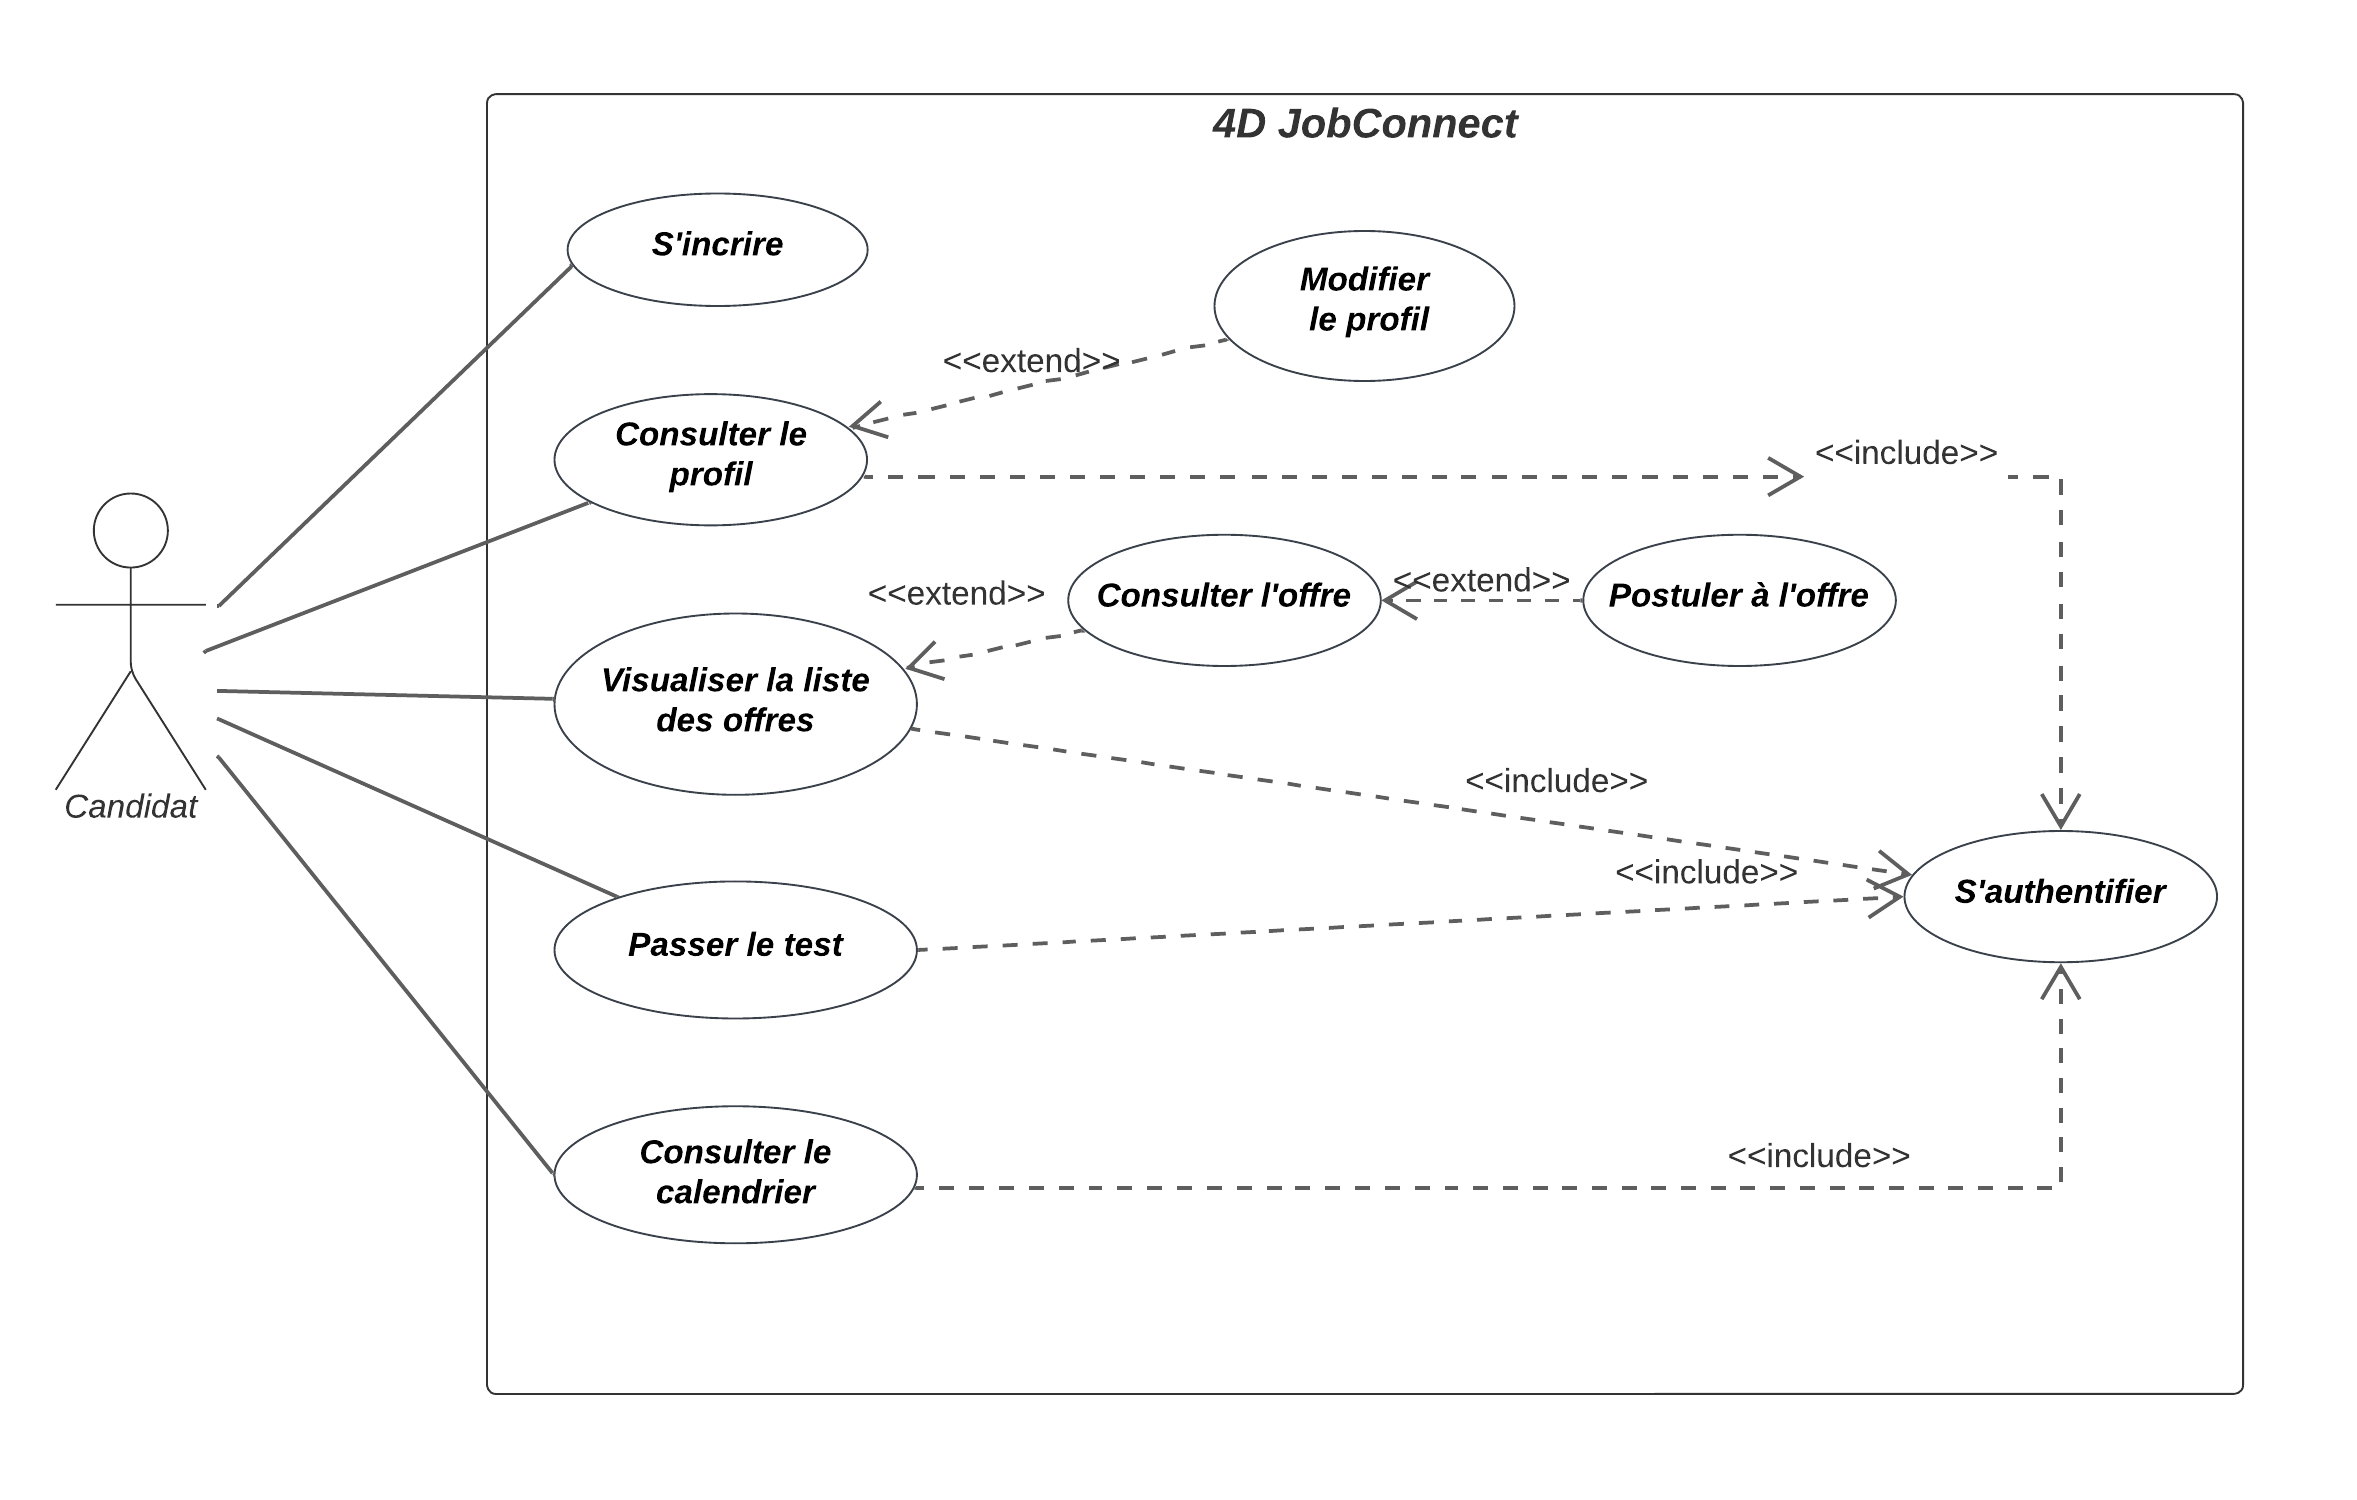
\includegraphics[scale=0.1]{Images/uc cand.png} % Replace with the actual filename of the IBM logo image
    \caption{Diagramme de cas d’utilisation du candidat}
    \label{fig:UCCandidat}
\end{figure}
\vspace{1cm}

\subsection{Diagramme de cas d’utilisation du recruteur}
\begin{figure}[h]
    \centering
    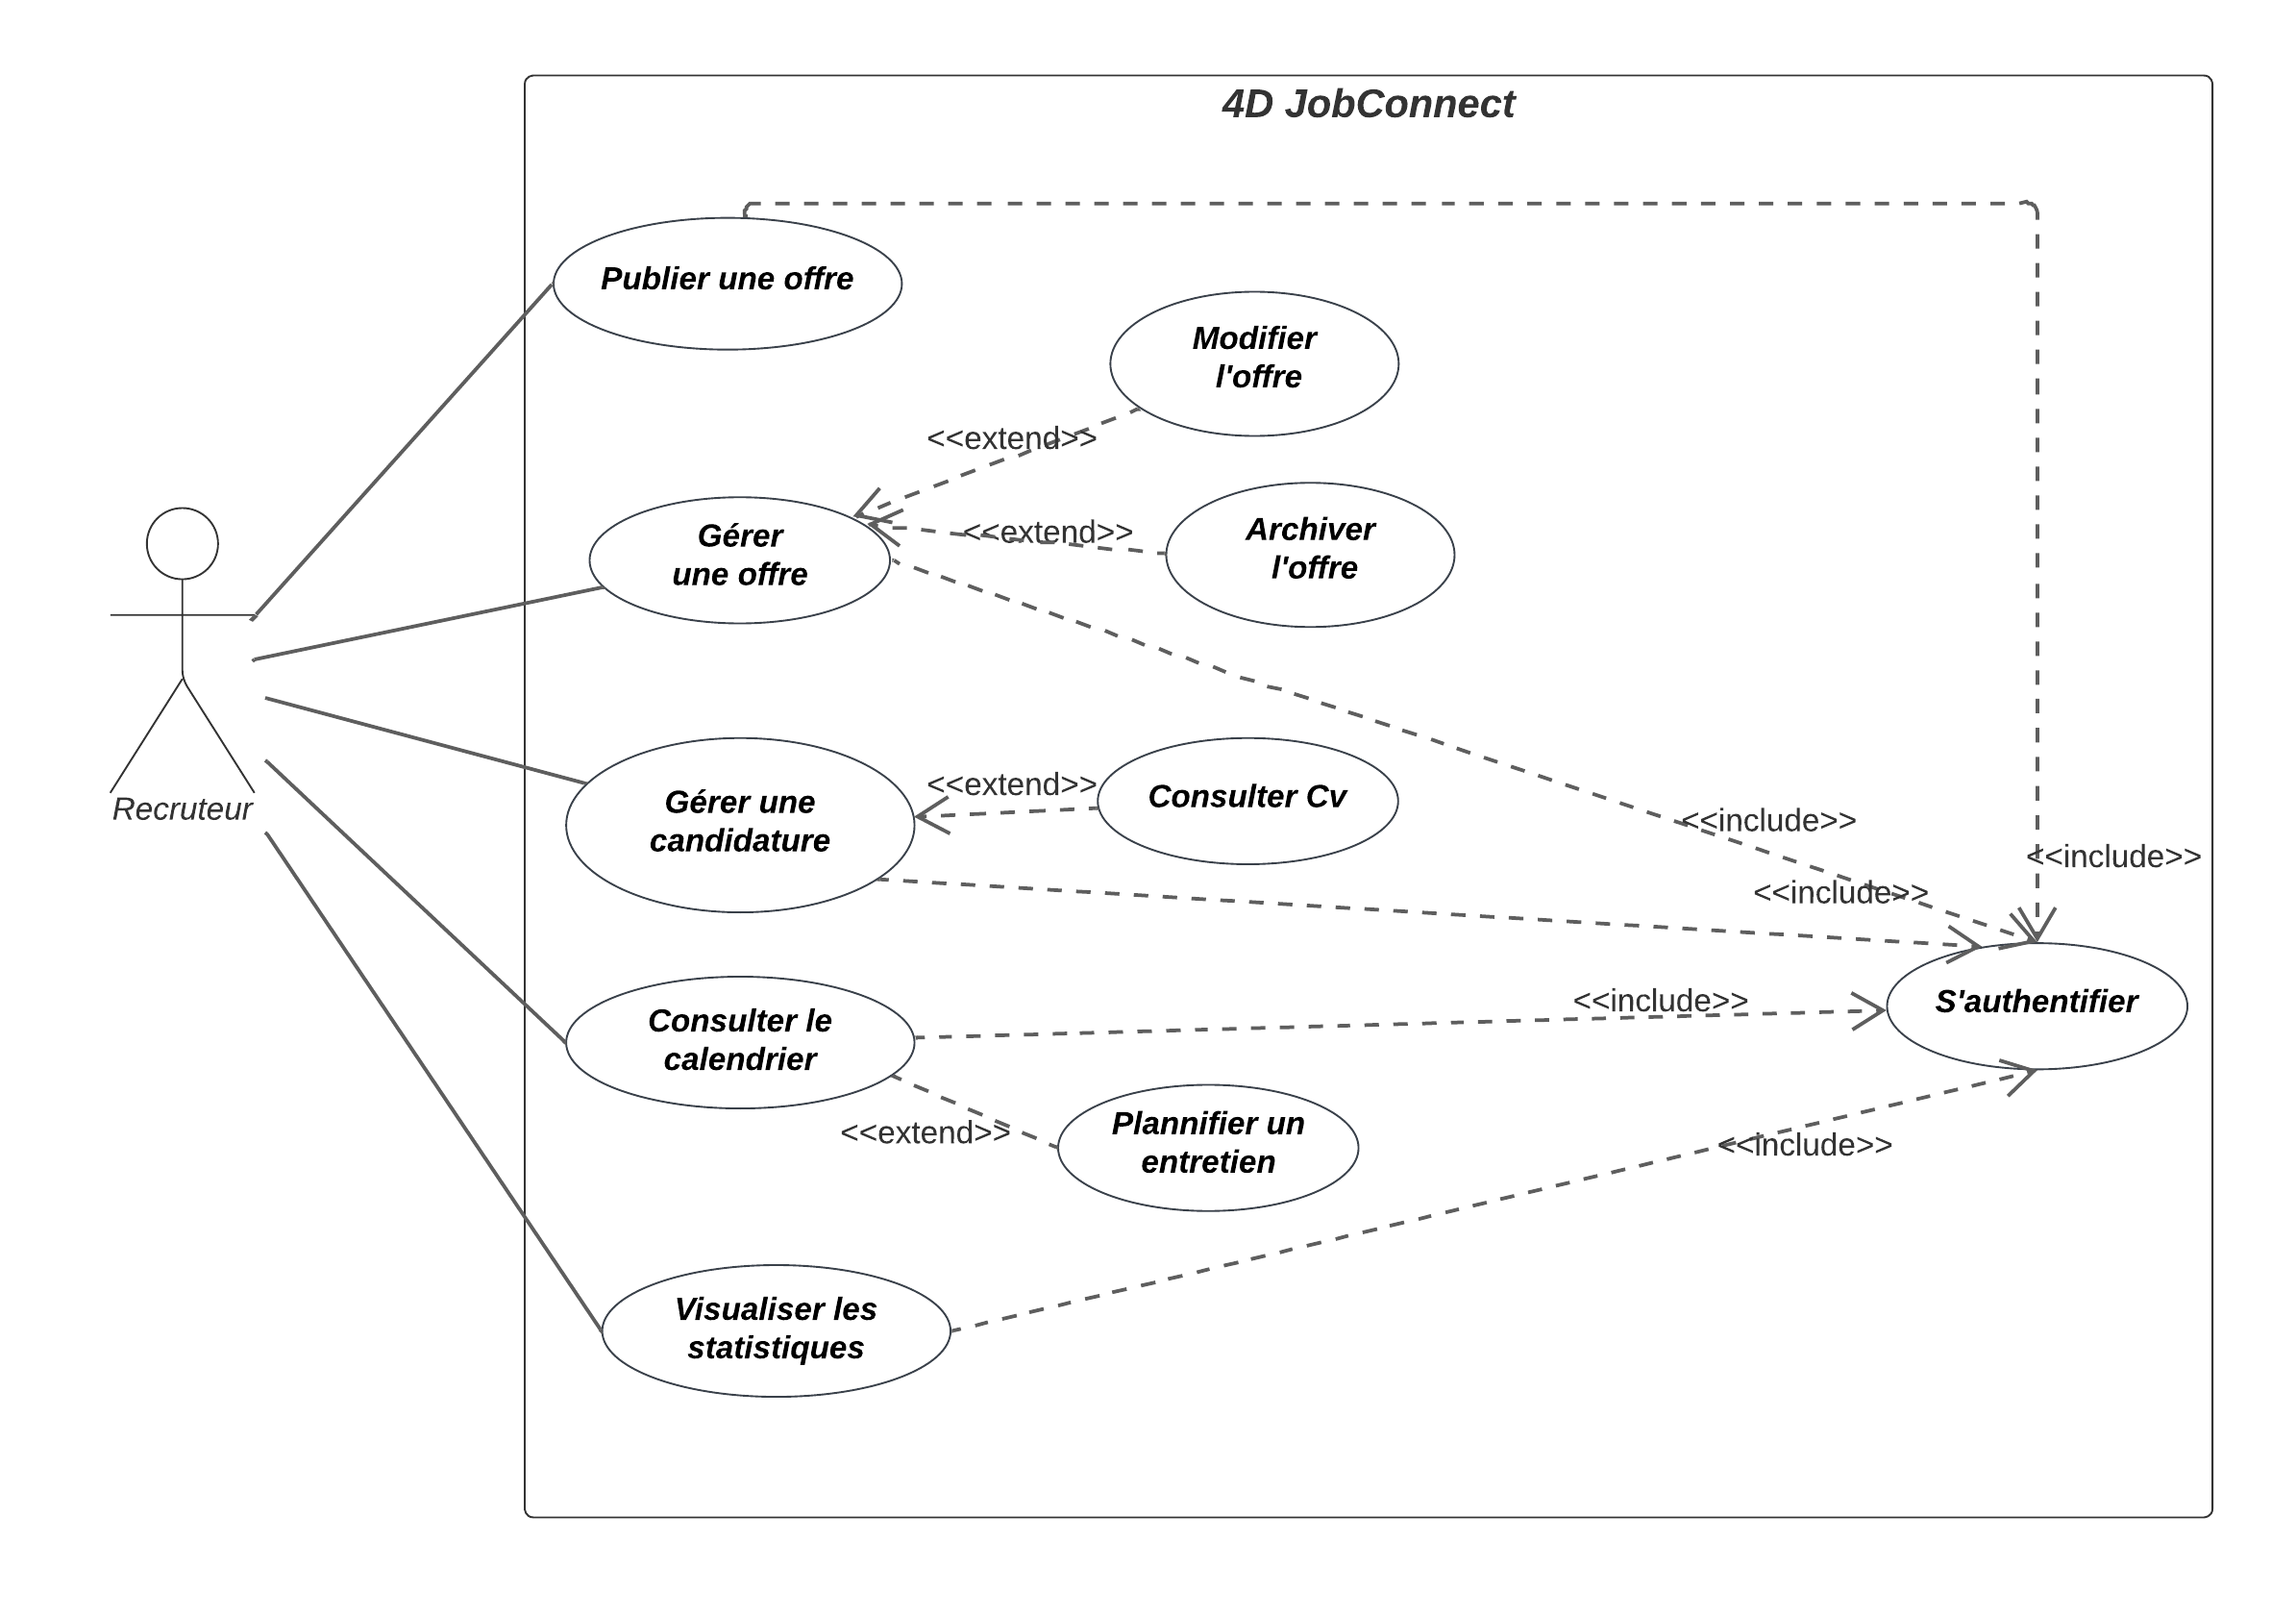
\includegraphics[scale=0.1]{Images/uc rec.png} % Replace with the actual filename of the IBM logo image
    \caption{Diagramme de cas d’utilisation du recruteur}
    \label{fig:UCRecruteur}
\end{figure}
\vspace{1cm}

\subsection{Diagramme de cas d’utilisation de l'administrateur}
\begin{figure}[htbp]
    \centering
    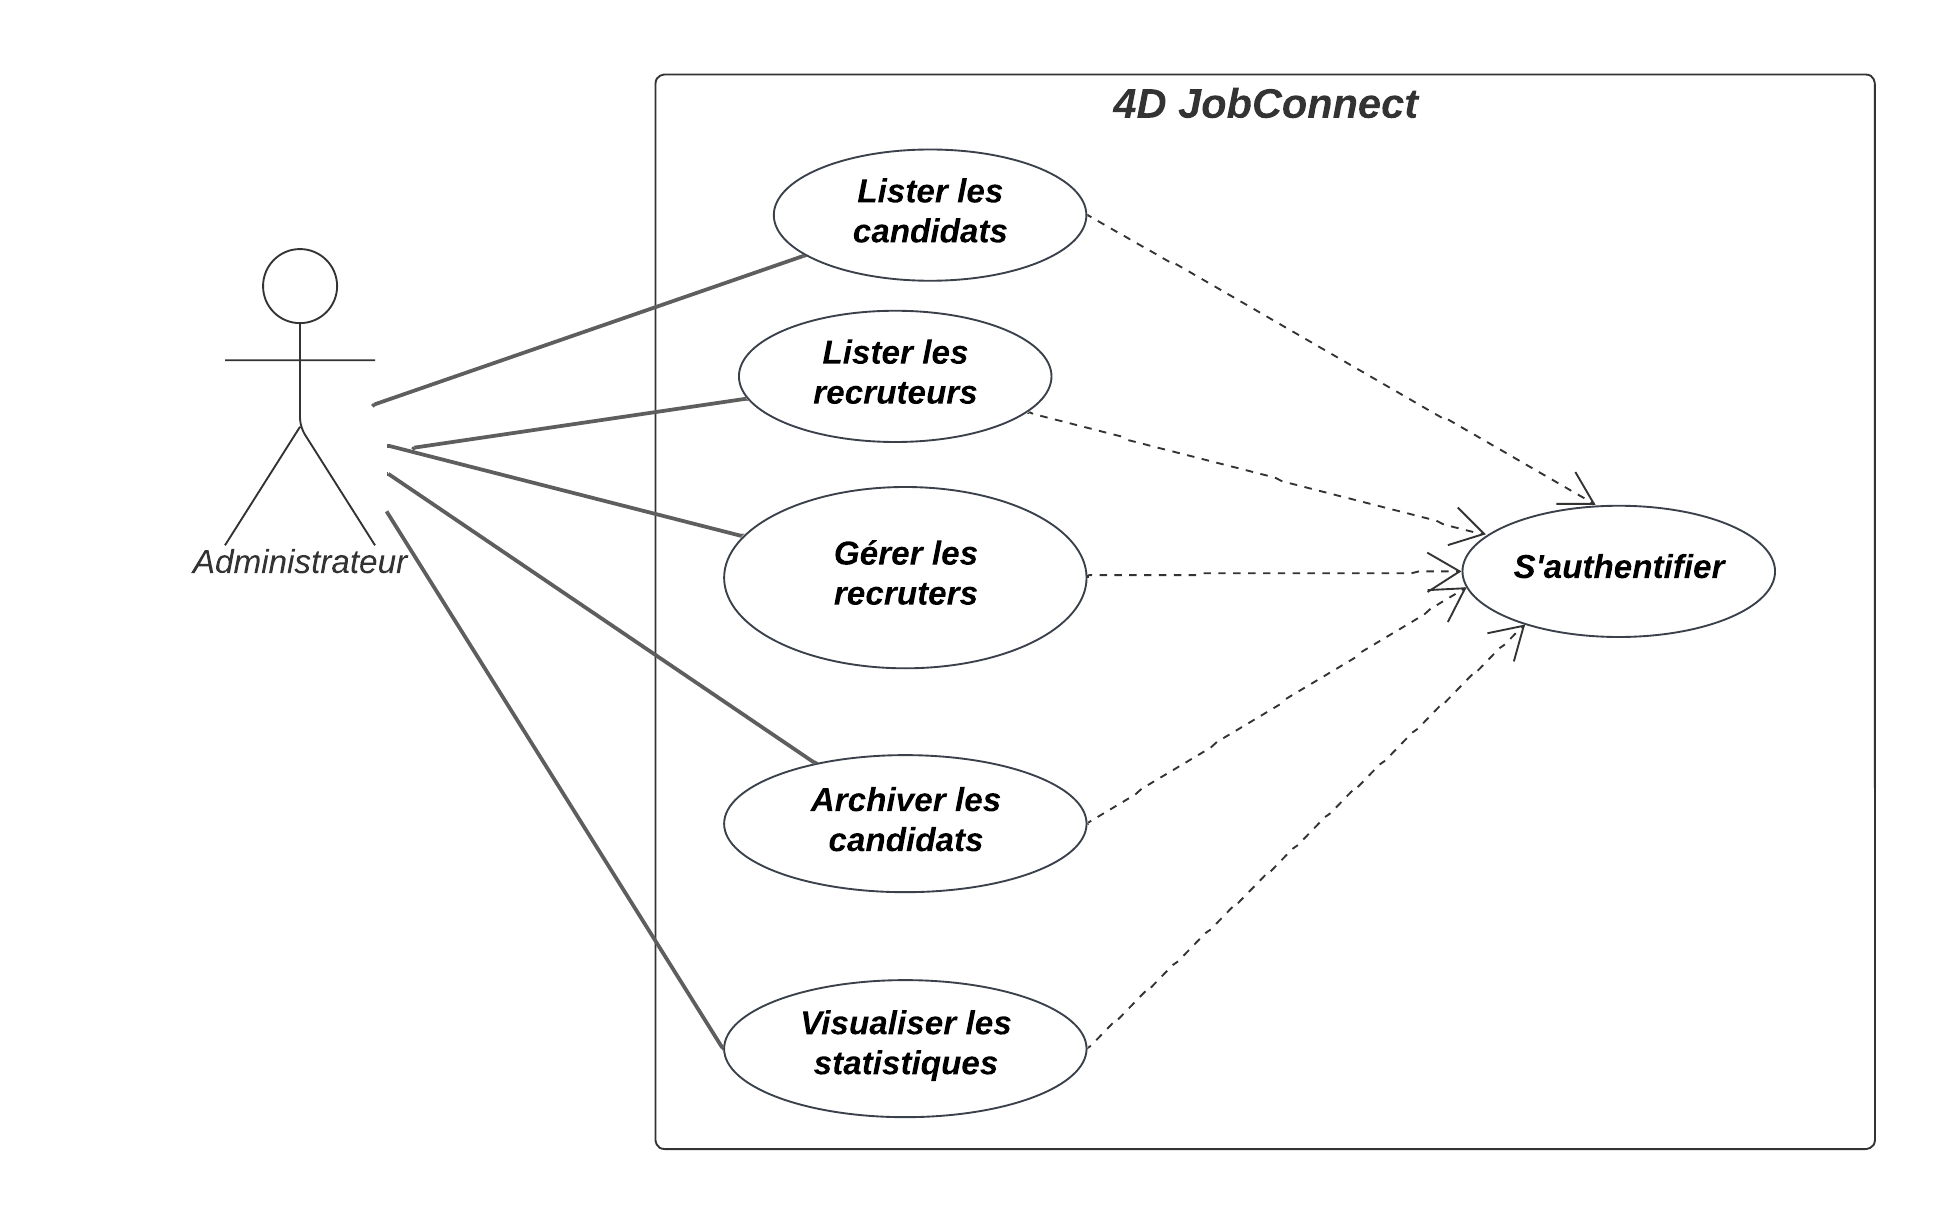
\includegraphics[scale=0.55]{Images/admin uc.png} % Replace with the actual filename of the IBM logo image
    \caption{Diagramme de cas d’utilisation de l'administrateur}
    \label{fig:UCAdmin}
\end{figure}
\vspace{1cm}

% Description textuelle
\section{Description textuelle des cas d'utilisation}

Afin de rendre notre diagramme de cas d’utilisation plus lisible et 
de mieux décrire le comportement du système, il est recommandé 
d'utiliser la description textuelle des cas d’utilisation. 
Cette approche permet de détailler de manière claire et structurée 
les interactions entre les acteurs et le système.

\subsection{Description textuelle : Publier une offre}
\begin{minipage}{\textwidth}
    \begin{table}[H]
    \centering
    \caption{Description Textuelle du Cas d'Utilisation "Publier une offre par le recruteur"}
    \begin{tabular}{| m{8cm} | m{8cm} |}
    \hline
    \multicolumn{2}{|c|}{\textbf{UC 1:} Publier une offre par le recruteur} \\ \hline
    \textbf{Acteur} & Recruteur \\ \hline
    \textbf{But} & Permettre à un recruteur de publier une nouvelle offre d'emploi sur la plateforme. \\ \hline
    \textbf{Préconditions} & \textbf{Postconditions} \\ \hline
    - Être authentifié en tant que recruteur. & - Une nouvelle offre est publiée sur la plateforme. \\ \hline
    \textbf{Scénario Principal} & \textbf{Scénario Alternatif} \\ \hline
    \begin{enumerate}
        \item Se connecter en tant que recruteur.
        \item Accéder à l'interface de publication des offres.
        \item Remplir les informations de l'offre : titre, description, compétences requises, localisation, etc.
        \item Publier l'offre sur la plateforme.
    \end{enumerate} & 
    \begin{enumerate}
        \item Le recruteur rencontre un problème de connexion.
        \item Le recruteur ne remplit pas tous les champs obligatoires.
        \item La publication de l'offre échoue en raison d'une erreur technique.
    \end{enumerate} \\ \hline
    \end{tabular}
    \label{tab:UCPublier_Offre}
    \end{table}
\end{minipage}

\subsection{Description textuelle : Postuler à une offre}

\begin{minipage}{\textwidth}
    \begin{table}[H]
    \centering
    \caption{Description Textuelle du Cas d'Utilisation "Postuler à une offre par le candidat"}
    \begin{tabular}{| m{8cm} | m{8cm} |}
    \hline
    \multicolumn{2}{|c|}{\textbf{UC 2:} Postuler à une offre par le candidat} \\ \hline
    \textbf{Acteurs} & Candidat \\ \hline
    \textbf{But} & Permettre à un candidat de postuler à une offre d'emploi disponible sur la plateforme. \\ \hline
    \textbf{Préconditions} & \textbf{Postconditions} \\ \hline
    - Être authentifié en tant que candidat. & - La candidature est soumise avec succès. \\ 
    - Documents requis téléversés dans le profil. & \\ \hline
    \textbf{Scénario Principal} & \textbf{Scénario Alternatif} \\ \hline
    \begin{enumerate}
        \item Se connecter en tant que candidat.
        \item Consulter les offres d'emploi disponibles.
        \item Sélectionner une offre qui correspond à ses compétences et intérêts.
        \item Cliquer sur le bouton "Postuler".
        \item Télécharger et soumettre les documents requis.
    \end{enumerate} & 
    \begin{enumerate}
        \item Problème de connexion.
        \item Aucune offre ne correspond à ses critères.
        \item Les documents requis ne sont pas téléversés :
            \begin{enumerate}
                \item Redirection vers la page de modification du profil pour téléverser les documents.
            \end{enumerate}
        \item Erreur technique lors de la soumission de la candidature.
    \end{enumerate} \\ \hline
    \end{tabular}
    \label{tab:UCPostuler_Offre}
    \end{table}
\end{minipage}

\subsection{Description textuelle : Passer le test}
\begin{minipage}{\textwidth}
    \begin{table}[H]
    \centering
    \caption{Description Textuelle du Cas d'Utilisation "Passer le test"}
    \begin{tabular}{| m{8cm} | m{8cm} |}
    \hline
    \multicolumn{2}{|c|}{\textbf{UC 3:} Passer le test} \\ \hline
    \textbf{Acteurs} & Candidat \\ \hline
    \textbf{But} & Permettre à un candidat de passer un test en ligne lié à une offre d'emploi. \\ \hline
    \textbf{Préconditions} & \textbf{Postconditions} \\ \hline
    - Avoir un score de CV supérieur au seuil défini.\\
    - Avoir déjà postulé à l'offre correspondante. & - Le test est passé avec succès. \\ \hline
    \textbf{Scénario Principal} & \textbf{Scénario Alternatif} \\ \hline
    \begin{enumerate}
        \item Être authentifié en tant que candidat.
        \item Consulter les offres d'emploi deja postulé
        \item Sélectionner une offre à laquelle le candidat a déjà postulé.
        \item Cliquer sur le bouton "Passer le test".
        \item Répondre aux questions du test en ligne.
        \item Soumettre les réponses.
    \end{enumerate} & 
    \begin{enumerate}
        \item Score de CV inférieur au seuil.
        \item Le candidat n'a pas encore postulé à l'offre correspondante.
        \item Problème technique lors du passage du test.
    \end{enumerate} \\ \hline
    \end{tabular}
    \label{tab:UCPasser_Test}
    \end{table}
\end{minipage}


\section*{Conclusion}
Ce chapitre aborde une phase essentielle pour l'étude et l'analyse 
de notre application. Nous y avons défini les différents besoins 
fonctionnels et non fonctionnels, présenté les diagrammes de cas 
d’utilisation, ainsi que leurs descriptions textuelles. Le chapitre 
suivant se concentrera sur la conception de notre solution en 
s'appuyant sur la concecption des maquettes, la détermination de 
l'architecture de notre système, et la modélisation les diagrammes de séquence et les diagrammes de 
classes.
